\documentclass[tikz,border=2pt]{standalone}
\usepackage{amsmath,amssymb}
\usepackage{tikz}
\usetikzlibrary{arrows.meta}

\begin{document}
% Near x0 a differentiable f acts like its derivative L = Df(x0): a small square grid around
% x0 is carried to a grid of parallelograms around f(x0), up to an error of order o(||h||).
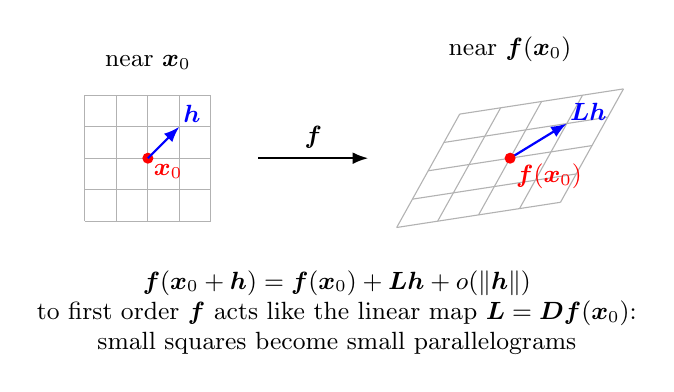
\begin{tikzpicture}[every node/.style={font=\small}, >={Latex[length=2mm]}]
	\foreach \i in {-2,...,2} {
		\draw[gray!60] (\i*0.4,-0.8) -- (\i*0.4,0.8);
		\draw[gray!60] (-0.8,\i*0.4) -- (0.8,\i*0.4);
	}
	\fill[red] (0,0) circle (2pt) node[below right, inner sep=2pt] {$\boldsymbol{x}_0$};
	\draw[->, blue, thick] (0,0) -- (0.4,0.4) node[above right, inner sep=1pt] {$\boldsymbol{h}$};
	\node[anchor=south] at (0,1.0) {near $\boldsymbol{x}_0$};
	\draw[->, thick] (1.4,0) -- (2.8,0) node[midway, above] {$\boldsymbol{f}$};
	\begin{scope}[xshift=4.6cm, cm={1.3,0.2,0.5,0.9,(0,0)}]
		\foreach \i in {-2,...,2} {
			\draw[gray!60] (\i*0.4,-0.8) -- (\i*0.4,0.8);
			\draw[gray!60] (-0.8,\i*0.4) -- (0.8,\i*0.4);
		}
		\draw[->, blue, thick] (0,0) -- (0.4,0.4);
	\end{scope}
	\fill[red] (4.6,0) circle (2pt) node[below right, inner sep=2pt] {$\boldsymbol{f}(\boldsymbol{x}_0)$};
	\node[blue, above right, inner sep=1pt] at (5.32,0.44) {$\boldsymbol{L}\boldsymbol{h}$};
	\node[anchor=south] at (4.6,1.1) {near $\boldsymbol{f}(\boldsymbol{x}_0)$};
	\node[anchor=north, align=center] at (2.4,-1.3) {$\boldsymbol{f}(\boldsymbol{x}_0+\boldsymbol{h})=\boldsymbol{f}(\boldsymbol{x}_0)+\boldsymbol{L}\boldsymbol{h}+o(\|\boldsymbol{h}\|)$\\ to first order $\boldsymbol{f}$ acts like the linear map $\boldsymbol{L}=\boldsymbol{Df}(\boldsymbol{x}_0)$:\\ small squares become small parallelograms};
\end{tikzpicture}
\end{document}
